\subsection{Architettura}
In questa sezione dar\`{o} una visione generale sull\textquoteright{}architettura dell\textquoteright{}applicativo. Il software presenta chiaramente una suddivisione in macrocomponenti, ovvero l\textquoteright{}interfaccia grafica (View), la business logic (Model) e l\textquoteright{}application logic. L\textquoteright{}application logic riceve comandi dalla View e interagisce se necessario con gli altri componenti. Il Model fornisce i metodi per accedere ai dati utili all\textquoteright{}applicazione. La View non interagisce in nessun modo con le componenti appartenenti al Model, ma solo con interfacce appartenenti alle componenti dell\textquoteright{}application logic. Il macrocomponente che presenta pi\`{u} sottocomponenti \`{e} l\textquoteright{}application logic; questo presenta classi di servizio e classi che effettuano operazioni logiche. Parte dei controlli sull\textquoteright{}inserimento dei dati da parte dell\textquoteright{}utente sono gestiti dalla View. Ogni elemento appartenente alla View eredita da una classe chiamata \textit{XView.java}; i principali elementi grafici: label, textbox, tabelle, form appartengono tutti alla stessa classe, \textit{XComponent.java}; un oggetto di tipo \textit{XComponent} presenta tra gli attributi un campo di tipo stringa che ne indica il tipo; l\textquoteright{}applicativo presenta dei file di tipo XML in cui viene definita la struttura di ogni form; i file che rappresentano la View vengono caricati dinamicamente al fine di eseguirne il parser e creare quindi gli oggetti di tipo \textit{XComponent} necessari. Nella struttura vengono definiti anche i nomi degli eventi che verrano invocati, ovvero i metodi che si occupano di gestire le operazioni dell\textquoteright{}utente. Lo svantaggio principale \`{e} l\textquoteright{}assenza di uno schema di riferimento da seguire per creare file che definiscono la struttura della View. Gli eventi vengono gestiti da degli script: nel momento in cui viene creato un oggetto di tipo \textit{XComponent}, ad esso vengono registrati se richiesto gli eventi; il comportamento di OnePointProject al verificarsi di un evento \`{e} il seguente: intercettazione dell\textquoteright{}evento da parte della classe, \textit{XInterpreter.java}, questa si occupa di richiamare il file di script indicato dall\textquoteright{}evento. Un file di script ha estensione \textit{jes}, contiene dei metodi e del codice Java, non contiene indicazioni in merito ai tipi dell\textquoteright{}oggetto, quindi se si invocano metodi su una certa variabile si deve assumere che quella variabile sia del tipo giusto. La funzione principale di questi script consiste in operazioni di recupero dati e di controllo. Gli script vengono interpretati da un compilatore ad hoc definito da OnePointProject che richiama alla fine azioni eseguite da classi \textit{Java}. I file di script che necessitano operazioni di caricamento di nuovi form o operazioni che necessitano interazioni con il database invocano una richiesta inglobata in un oggetto di tipo \textit{XMessage} che ha come attributi il nome del servizio da invocare, il rispettivo metodo e eventualmente i parametri necessari richiesti dalla firma del metodo richiesto. Concludendo l\textquoteright{}applicativo presenta una struttura le cui modifiche in aggiunta non sono difficili da sviluppare, ma richiedono tempo per la loro integrazione con gli altri componenti. 

\subsection{Database}
L\textquoteright{}applicativo per relazionarsi con il database utilizza Hibernate. Il file di mapping viene creato in modo automatico utilizzando dei file XML. L\textquoteright{}applicativo predisponde dei file XML per ogni classe i cui oggetti \`{e} necessario rendere persistenti. Questi file purtroppo non hanno uno schema predefinito da seguire e quindi obbligano il programmatore estraneo al team di sviluppo ad attenersi ai file gi\`{a} presenti in caso di modifiche o aggiunte da parte di quest\textquoteright{}ultimo. Il tutto \`{e} molto comodo, ma il principale svantaggio di questa scelta implementativa \`{e} che le classi Java presentano delle dipendenze cicliche. Tra breve dar\`{o} una spiegazione a riguardo; in OnePointProject possono presentarsi tre casi, che ora illustrer\`{o}.

\subparagraph{Attributo il cui tipo non \`{e} definito dall\textquoteright{}utente} \quad \quad \\ \\
La sintassi da utilizzare sar\`{a} la seguente: \\
\textit{<field name=''Nome\_attributo'' type=''Tipo\_attributo''/>}; \\
Per esempio se nella classe \`{e} presente la dichiarazione: \textit{private String nome}, sar\`{a} sufficiente riportare nel file XML: \\
\textit{<field name=''nome'' type=''String''/>}.

\subparagraph{Attributo il cui tipo \`{e} un tipo composto} \quad \quad \\ \\
Si tratta di un tipo utilizzato per raccogliere un certo numero di attributi di tipo semplice, ad esempio \`{e} il caso dell\textquoteright{}indirizzo. Per esempio una classe dichiara una variabile di tipo \textit{Indirizzo}, che presenta i seguenti attributi di tipo semplice: \textit{via, numero civico, paese}.
La sintassi da utilizzare sar\`{a} la seguente:\\
\textit{<composite name=''nome attribuito al tipo composto'' type=''tipo della classe composta''>} \\
\textit{<field name=''Nome attributo java'' column=''Nome attributo colonna nel database'' type=''Tipo dell\textquoteright{}attributo''/>} \\
\textit{</composite>}.\\
Ovviamente, e questo vale per tutte le casistiche, il tag field pu\`{o} essere accompagnato dall\textquoteright{}impostazione di alcune propriet\`{a}, ad esempio se l\textquoteright{}attributo deve essere richiesto o meno nel db \textit{(mandatory=``true\textquoteright{}\textquoteright{})}, se l\textquoteright{}attributo deve essere ordinabile \textit{(ordered=''true'')} ecc. Nel database tutti gli attributi del tipo composto sono inglobati come attributi della tabella nella cui classe \`{e} stata indicata una dipendenza nei confronti del tipo composto, non verr\`{a} quindi realizzata una tabella a se stante rappresentante l\textquoteright{}entit\`{a} del tipo composto.

\subparagraph{Relazioni tra entit\`{a}} \quad \quad \\ \\
Si ha quindi una dipendenza tra tipi, nel database viene espressa con relazioni del tipo \textit{1:1, 1:n, m:n}. Le relazioni \textit{m:n} vengono scomposte in 2 relazioni di tipo \textit{1:n} introducendo una nuova relazione. A questo corrisponde anche una classe Java, in questo modo ad ogni relazione corrisponder\`{a} sempre una classe Java.\\
Riporto qui un esempio del tipo di relazione in questione: \\
nella classe \textit{OpActivity.java} si ha la seguente dichiarazione: \textit{private OpProjectPlan projectplan}; nel file XML corrispondente alla classe OpActivity.java \`{e} presente il seguente tag: \\
\textit{<relationship name=''ProjectPlan'' type=''OpProjectPlan'' back-relationship=''Activities''/>}
Quindi occorre indicare il nome dell\textquoteright{}attributo, il tipo e la relazione; nel file XML corrispondente alla classe OpProjectPlan.java \`{e} definito un tag che a seconda del tipo di relazione \textit{1:1 o 1:n} sar\`{a} rispettivamente: \\
\textit{<relationship name=''Activities'' type=''OpActivity'' back-relationship=''ProjectPlan''/>}, oppure \\
\textit{<relationship name=''Activities'' type=''OpActivity'' collection-type=''Set'' \\ back-relationship=''ProjectPlan'' cascade=''delete''/>}.\\
L\textquoteright{}attributo name si deve riferire ad un attributo della classe Java corrispondente; in questo modo si presentano delle dipendenze cicliche. La classe \textit{OpProjectPlan.java} presenta un attributo che \`{e} una collezione di oggetti di tipo \textit{OpActivity} e la classe \textit{OpActivity.java} presenta un riferimento all\textquoteright{}oggetto di tipo \textit{OpProjectPlan} corrispondente. Questo scelta potrebbe portare a delle inconsistenze di dati a \textit{run-time}.

\begin{figure}[H]
\begin{center}
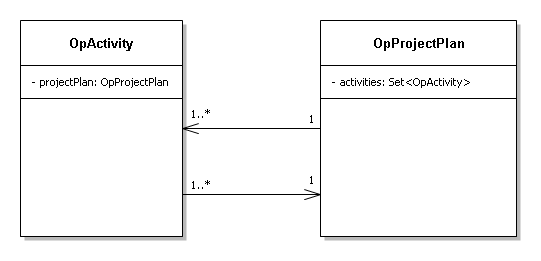
\includegraphics[width=1\textwidth]{img/DipendenzaCiclica.png}
\caption{Esempio di dipendenza ciclica}
\label{fig:Esempio di dipendenza ciclica}
\end{center}
\end{figure}
